\hypertarget{ux6b22ux8fceux4f7fux7528ux4f18ux8003ux8bd5ux5728ux7ebfux8003ux8bd5ux7cfbux7edf}{%
\section{欢迎使用优考试在线考试系统}\label{ux6b22ux8fceux4f7fux7528ux4f18ux8003ux8bd5ux5728ux7ebfux8003ux8bd5ux7cfbux7edf}}

1{[}单选题{]}食醋是什么味道的?

A.酸

B.甜

C.苦

D.辣

{[}答案{]}A {[}分数{]}5 {[}分类{]}全民闯关 {[}标签{]}常识,简单

{[}解析{]}

2{[}单选题{]} 函数\(y = \lg\frac{x}{x - 2} + \arcsin\frac{x}{3}\)
的定义域是\_\_\_\_\_\_\_。

A. \(\left\lbrack - 3,\ \ 0 \right) \cup (2,\ 3\rbrack\)

B. \(\lbrack - 3,\ 3\rbrack\)

C. \(\left\lbrack - 3,\ 0 \right)\  \cup \ \ (1,\ 3\rbrack\)

D. \(\left\lbrack - 2,\ 0 \right) \cup (1,\ 2)\)

{[}答案{]}A {[}分数{]}4 {[}分类{]}数学 {[}标签{]}很难

{[}解析{]}

3{[}单选题{]} I was very interested in\_\_\_\_\_\_\_ she told me .

A. all that

B. all which

C. all what

D. that

{[}答案{]} A {[}分数{]}4 {[}分类{]}数学 {[}标签{]}很难

{[}解析{]}我对她告诉我的所有事情都非常感兴趣。定语从句,在定语从句中,当先行词为all,
something,anything等不定代词时,关系词要用that,而不用which,分析句子结构可知,空处作in的宝语。再结合选项,
all为先行词,应用关系代词that引导定语从句。故选A

4{[}多选题{]} 一年中有几个季节?

A.春 B.夏

C.秋 D.冬

{[}答案{]}ABCD {[}分数{]} 5 {[}分类{]}生活常识 {[}标签{]}简单

{[}解析{]}

5{[}不定项选择题{]}是《红楼梦》中的人物有( )

A.王熙凤 B.贾宝玉 C.林黛玉

D.薛宝钗 E.貂蝉

{[}答案{]}ABCD {[}分数{]}5 {[}分类{]}文学 {[}标签{]}简单

{[}解析{]}

6{[}不定项选择题{]}如果你是传说人物``白娘子''的助理,你一定不会让她喝什么?

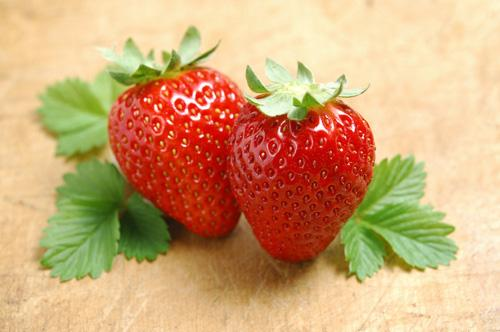
\includegraphics[width=2.01757in,height=1.33962in]{cache/image/media/image1.jpeg}

A.雄黄酒 B.老白干 C.红酒

{[}答案{]}A {[}分数{]}5 {[}分类{]}全民闯关 {[}标签{]}简单

{[}解析{]}

7{[}判断题{]}荔枝多吃上火?

A.对 B.错

{[}答案{]}A {[}分数{]}5 {[}分类{]}生活常识 {[}标签{]}简单

{[}解析{]}

8{[}判断题{]}马铃薯是果实?

A. √ B. ×

{[}答案{]}B {[}分数{]}5 {[}分类{]}生活常识 {[}标签{]}常识,简单

{[}解析{]}马铃薯是是蔬菜。

9{[}填空题{]}一根绳子两个头,三根半绳子有( )个头?

A.8

{[}答案{]}~ {[}分数{]}5~ {[}分类{]}生活常识~ {[}标签{]}常识,简单\\
{[}解析{]}

~

10{[}填空题{]}一年有\_\_\_\_\_个月,有\_\_\_\_\_天,有\_\_\_\_\_个季节?

A.12 =\textgreater2

B.365 =\textgreater2

C.4=\textgreater1\\
{[}答案{]}~~{[}分数{]}5~~~{[}分类{]}系统功能~ {[}所有空无序{]}
{[}标签{]}常识,地理\\
{[}解析{]}~~~
